\section{Parallel Design}\label{sec:parallel}

Sequential WFC exhibits a strict dependency between successive collapses: each
collapse modifies the superposition set of adjacent chunks, conditioning future
choices. This dependency makes parallelism non-trivial to extract, as a naïve
parallelization in which multiple chunks are collapsed simultaneously without
coordination can produce contradictory states or violate the adjacency
constraints defined by the model.

The approach described here resolves this problem through a decomposition of the
domain into nodes and a policy of exclusive access to chunks via mask sliding,
which guarantees by construction the absence of conflicts between concurrent
collapses. The result is an algorithm in which all nodes advance in parallel
synchronously, each operating in isolation on its own subdomain, with
communications exclusively local to immediate geometric neighbors.

% 1 image representing the mask and chunks

The main properties of the implementation are the following:

\begin{itemize}
    \item \textbf{Statistical correctness:} The parallel output is statistically
    equivalent to the sequential one that is, it belongs to the same distribution
    of valid configurations while not being deterministically identical given the
    same seed, as the global order of collapses differs between the two formulations.

    \item \textbf{Communication locality:} Each node communicates exclusively with
    its immediate geometric neighbors. No global communications are present during
    the collapse phase, with the exception of barrier synchronizations between
    successive slides.

    \item \textbf{Architecture independence:} The adopted parallelism model makes
    no assumptions about the underlying hardware: the decomposition into nodes is
    applicable to distributed-memory systems via MPI, shared-memory systems via
    threads, and hybrid models alike.

    \item \textbf{Conflict-free by construction:} The geometry of the sliding
    guarantees that no chunk is ever covered simultaneously by two distinct masks,
    eliminating the need for locking mechanisms or runtime conflict resolution.
\end{itemize}

For this implementation we define the following elements:

\begin{description}
    \item[Node:] A set of $3 \times 3$ chunks whose evolution is managed by a
    single MPI process or thread. The node is the unit of work of the parallel
    system: it performs the collapse of its own chunks and manages the exchange
    of updates with adjacent nodes.

    \item[Mask:] A $3 \times 3$ chunk window centered on the chunk currently
    being collapsed. It defines the set of chunks that may be influenced by the
    propagation originating from the current collapse, potentially extending onto
    chunks belonging to adjacent nodes.
\end{description}
\begin{figure}[ht]
\centering
\adjustbox{max width=\textwidth}{
\setlength{\fboxsep}{10pt} % imposta il padding a 10pt
\fbox{
\begin{minipage}{0.6\linewidth}
    \centering
    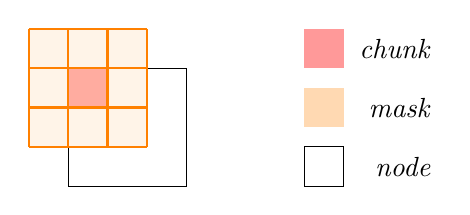
\begin{tikzpicture}[scale=0.5]
    
    \draw[step=1cm, black, thin] (0,0) rectangle (3,3);
    % evidenzio un pixel (0,0)
    \fill[red!40] (0,2) rectangle ++(1,1);
    \fill[orange!30, opacity=0.3] (-1,1) rectangle ++(3,3);
    \draw[step=1cm, orange, thick] (-1,1) grid ++(3,3);
    % legenda
    \fill[color=red!40] (6,3) rectangle ++(1,1);
    \node[anchor=east] at (9.5,3.5) {\textit{chunk}};
    \fill[color=orange!30] (6,1.5) rectangle ++(1,1);
    \node[anchor=east] at (9.5,2) {\textit{mask}};
    \draw[step=1cm, black, thin] (6,0) rectangle ++(1,1);
    \node[anchor=east] at (9.5,0.5) {\textit{node}};
\end{tikzpicture}
\end{minipage}
}}
\caption{Visual representation of chunk, mask and node}
\label{fig:uno}
\end{figure}

\paragraph{Mask sliding and update ordering}
The parallelism of the algorithm is founded on the geometric property by which
the masks of distinct nodes never overlap on the same chunk at the same instant.
To guarantee this property, the mask slides over the 9 chunks internal to the
node following a row-major ordering, visiting positions in sequence from the
bottom row to the top, left to right. At each sliding step, the mask is centered
on a different chunk, and the geometry of the system ensures that the current
chunk is not simultaneously covered by the mask of any adjacent node, making
the local collapse conflict-free.

% 2 image of the sliding masks


\begin{figure}[ht]
\centering
\adjustbox{max width=\textwidth}{
\setlength{\fboxsep}{10pt} 
\fbox{
\begin{minipage}{0.8\linewidth}
    \centering
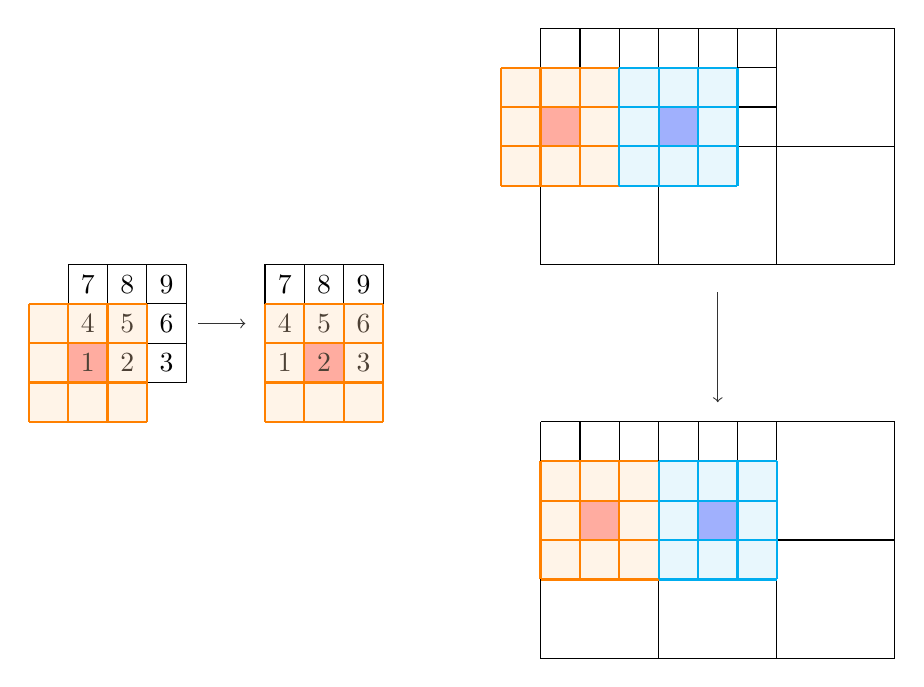
\begin{tikzpicture}[scale=0.5]
    \fill[red!40] (0,-6) rectangle ++(1,1);
    \node at (0.5,-5.5) {1};
    \node at (1.5,-5.5) {2};
    \node at (2.5,-5.5) {3};
    \node at (0.5,-4.5) {4};
    \node at (1.5,-4.5) {5};
    \node at (2.5,-4.5) {6};
    \node at (0.5,-3.5) {7};
    \node at (1.5,-3.5) {8};
    \node at (2.5,-3.5) {9};
    % griglia 7x7
    \draw[step=1cm, black, thin] (0,-6) grid (3,-3);
    % evidenzio un pixel (0,0)
    \fill[orange!30, opacity=0.3] (-1,-7) rectangle ++(3,3);
    \draw[step=1cm, orange, thick] (-1,-7) grid ++(3,3);

    \draw[->, black!80] (3.3,-4.5) -- (4.5,-4.5);

    % griglia 7x7
    \fill[red!40] (6,-6) rectangle ++(1,1);
    \node at (5.5,-5.5) {1};
    \node at (6.5,-5.5) {2};
    \node at (7.5,-5.5) {3};
    \node at (5.5,-4.5) {4};
    \node at (6.5,-4.5) {5};
    \node at (7.5,-4.5) {6};
    \node at (5.5,-3.5) {7};
    \node at (6.5,-3.5) {8};
    \node at (7.5,-3.5) {9};
    \draw[step=1cm, black, thin] (5,-6) grid (8,-3);
    % evidenzio un pixel (0,0)
    \fill[orange!30, opacity=0.3] (5,-7) rectangle ++(3,3);
    \draw[step=1cm, orange, thick] (5,-7) grid ++(3,3);

%% seconda parte !!!!
    \draw[step=1cm, black, thin] (18,0) rectangle (21,3);
    \draw[step=1cm, black, thin] (18,-3) rectangle (21,0);
    \draw[step=1cm, black, thin] (15,-3) rectangle (18,0);
    \draw[step=1cm, black, thin] (12,-3) rectangle (15,0);
    
    \fill[red!40] (12,0) rectangle ++(1,1);
    % griglia 7x7
    \draw[step=1cm, black, thin] (12,0) grid (15,3);
    % evidenzio un pixel (0,0)
    \fill[orange!30, opacity=0.3] (11,-1) rectangle ++(3,3);
    \draw[step=1cm, orange, thick] (11,-1) grid ++(3,3);

    \fill[blue!40] (15,0) rectangle ++(1,1);
    % griglia 7x7
    \draw[step=1cm, black, thin] (15,0) grid (18,3);
    % evidenzio un pixel (0,0)
    \fill[cyan!30, opacity=0.3] (14,-1) rectangle ++(3,3);
    \draw[step=1cm, cyan, thick] (14,-1) grid ++(3,3);

    \draw[->, black!80] (16.5,-3.7) -- (16.5,-6.5);
%% 2.2
\draw[step=1cm, black, thin] (18,-10) rectangle (21,-7);
    \draw[step=1cm, black, thin] (18,-13) rectangle (21,-10);
    \draw[step=1cm, black, thin] (15,-13) rectangle (18,-10);
    \draw[step=1cm, black, thin] (12,-13) rectangle (15,-10);
    \fill[red!40] (13,-10) rectangle ++(1,1);
    % griglia 7x7
    \draw[step=1cm, black, thin] (12,-10) grid (15,-7);
    % evidenzio un pixel (0,0)
    \fill[orange!30, opacity=0.3] (12,-11) rectangle ++(3,3);
    \draw[step=1cm, orange, thick] (12,-11) grid ++(3,3);

    \fill[blue!40] (16,-10) rectangle ++(1,1);
    % griglia 7x7
    \draw[step=1cm, black, thin] (15,-10) grid (18,-7);
    % evidenzio un pixel (0,0)
    \fill[cyan!30, opacity=0.3] (15,-11) rectangle ++(3,3);
    \draw[step=1cm, cyan, thick] (15,-11) grid ++(3,3);

\end{tikzpicture}
\end{minipage}
}}
\caption{Visualization of the mask sliding update order}
\label{fig:due}
\end{figure}

When the mask extends onto chunks belonging to a neighboring node, the owner
node sends a copy of those chunks to the node that needs to update them. The
latter performs the propagation, updates the received copies, and sends them
back to the owner before the next sliding step. The correctness of this exchange
is guaranteed by the fact that, by construction, the owner node does not cover
with its own mask the temporarily transferred chunks, eliminating any access
conflict.

All nodes advance synchronously: each sliding step is preceded by a global
synchronization phase in which each node sends and receives updates relative
to the chunks shared with its neighbors, after which it frees the memory of
chunks no longer needed for the subsequent iteration. Chunks that fall beyond
the boundaries of the global domain are simply ignored.

\subsection{Communication Pattern}
The communication pattern arising from mask sliding is local and point-to-point:
each node communicates exclusively with the geometric neighbors that share a
border or a vertex with it in the node grid.

Communications occur via asynchronous exchange, allowing the internal computation of the node to overlap
with the transfer of boundary data. The volume of data exchanged per
synchronization step is proportional to the number of chunks shared with each
neighbor, the full superposition set of each chunk that is, the set of
compatible patterns for each tile and the thickness of the boundary region
determined by the maximum extent of propagation.



\paragraph{Time Complexity}
Let $P$ be the number of nodes and $L$ the side length of a chunk in tiles.
Each node manages a $3 \times 3$ subdomain of chunks, and its local computation
is equivalent to running sequential WFC on $9 \cdot L^2$ cells. The time
complexity per node is therefore $\mathcal{O}(L^2 \cdot |T|^2 + L^2 |T|\log L)$,
identical to the sequential case scaled to the subdomain size.

Since all nodes advance synchronously and operate in isolation on disjoint
subdomains, the $P$ nodes execute their local computation in parallel, yielding
a parallel time complexity for the computation phase of:
\[
T_{comp}(N,P)=\mathcal{O}\left(\frac NP \cdot |T|^2 + \frac NP|T| \log \frac NP\right)
\]
where $N$ is the total number of cells in the domain. To this must be added
the synchronization overhead $T_{sync}$, incurred at each of the 9 sliding
steps. during which each node exchanges the superposition sets
of the chunks shared with its neighbors.

\[
    T_{sync}(N,P)=\mathcal{O}\left(\frac NP|T|\right)
\] 
In conclusion, the total time complexity for the parallel algorithm is the combination of $T_{comp}$ and $T_{sync}$
$$T(N,P)=T_{comp}(N,P)+T_{sync}(N,P)=\mathcal O\left(\frac NP \cdot |T|^2 + \frac NP |T|\log \frac NP\right)$$

\paragraph{Space Complexity}
Each node stores the superposition states of its $3 \times 3$ chunks, along with temporary copies of boundary chunks received from adjacent nodes. The local memory required to store these chunks is $18 L^2 \cdot |T|$. Combined with the 3-dimensional adjacency bit-matrix, the space complexity per node is $\mathcal{O}(L^2 \cdot |T|+|T|^2)$. Consequently, the total space requirement across all nodes is $\mathcal{O}(N \cdot |T|+P|T|^2)$.



        